%\newcommand{\nsubparagraph}[1]{\textbf{#1}}
\newcommand{\AVG}{\mathit{AVG}}

\section{Empirical Evaluation}\label{sec:empiricalEvaluation}
In this section all six identification strategies are analyzed in terms of their process to obtain the database
candidate set $R$ (retrieval step), their database set $r$ selection process, and their bijection $h$ production process
(identification) under varying amounts of false stars and Gaussian noise.
The main areas of interest here are the accuracy of each step, and the time to produce a result.

%For the figures given in the following section, ANG corresponds to the Angle method, INT to the Interior Angle method,
%SPH to the Spherical Triangle method, PLN to the Planar Triangle method, PYR to the Pyramid method,
%and COM to the Composite Pyramid method.

\subsection{Experimental Setup}\label{subsec:experimentalSetup}
\nsubparagraph{Star Database}
The astronomical catalog used to populate the $K$ database is the Hipparcos Input
Catalogue~\cite{perryman:hipparcosCatalogue}.
Entries that do not have a point $\left( \alpha, \delta \right)$ associated with it were not recorded, giving
$117{,}956$ total stars.
Out of this entire set, only $4{,}560$ are visible from Earth with the naked eye (apparent magnitude $m$ less than 6.0).
An additional constraint for each database $K^2, K^3, \bar{K^3}$ that all stars in each pair or trio be within 20
degrees of each other was placed to shorten each algorithm's $R$ retrieval running time.
A field-of-view between 10 to 20 degrees is common for most astronomy based CCD
cameras~\cite{mortari:pyramidIdentification}.
All sets $K^2, K^3, \bar{K^3}$ construct combinations and permutations using the $4{,}560$ elements and this field
of view constraint.
A constant radius was attached to each recorded $\left(\alpha, \delta \right)$, and was converted from this spherical
frame to a 3D Cartesian frame to construct the point $[ x \ y \ z ]$ for $K$.
%~\autoref{eq:sphereToCartesian} was used with
%each recorded $\left(\alpha, \delta \right)$ and $r \seq 1$, then normalized.

\nsubparagraph{Benchmark Data Generation}
Before a raw image can be used in any of the star identification algorithms presented above, it must go through
three major processes: blob detection, centroid determination, and a 2D $\rightarrow$ 3D transformation process.
If a blob is not wholly detected, the centroid is not determined correctly, or the transformation process
is not precise enough, error will exist as input to the algorithm prior to starting.
Given that our goal is to only characterize each star identification algorithm itself, the solution implemented here
involves generating artificial images in some quasi 3D space.

Prior to generating the benchmark data, three items are specified: a field of view $\psi$, a true attitude
$A^{\nicefrac{\iFrame}{\kFrame}}$, and a 3D vector $\vv{r_f}$ in the database frame $\kFrame$ that determines
the center of the image.
The next step is to find all nearby stars to the $\vv{r_f}$ in the database.
This is denoted as $J$:
\begin{equation}
    J = \set{ j \mid j \in K \land \theta\left( j, \vv{r_f} \right) < \frac{\psi}{2} }
\end{equation}
To get the $I$ set, each star in $J$ is then rotated by the true attitude $A^{\nicefrac{\iFrame}{\kFrame}}$:
\begin{equation}
    I = \set{ A^{\nicefrac{\iFrame}{\kFrame}} \cdot j \mid j \in J }
\end{equation}
The set $I$, the field of view, and the rotated image center
$\vv{b_f} \seq A^{\nicefrac{\iFrame}{\kFrame}} \cdot \vv{r_f}$ are then presented to each star identification algorithm.

The first type of noise exists as variance between the relative positions of stars represented in the database and those
represented in the image.
This may come from misidentifying the centroids in the image or out-of-date databases.
To introduce Gaussian noise to an image, we spherically linearly interpolate each star toward some random 3D vector on
the unit sphere (\textit{SLERP}) and distribute the magnitude of the movement normally.
To describe our noise independent of this random vector, we divide a normal random variable by the current angular
separation between both stars.
Given a star $b_i\!\in\!I$, Gaussian noise is applied to obtain the distributed vector $b'_i$~\cite{kremer:slerp}:
\begin{equation}
    b'_i = \frac{\sin (1 - K)\Omega}{\sin \Omega}b_i + \frac{\sin \left( K \Omega \right)}{\sin \Omega}b^\star_i
\end{equation}
\begin{subequations}
    where $b^\star_i$ represents some random vector with uniformly distributed elements, $\Omega$ describes the
    angle subtended by the arc, and $K$ describes the magnitude of the interpolation.
    Below, $\rho$ represents the standard deviation of noise.
    \begin{align}
            b^\star_i &= \left[ \sim U(-1, 1), \sim U(-1, 1), \sim U(-1, 1) \right] \\
            \Omega &= \arccos \left ( b^{\star}_i \cdot b_i \right) \\
            K &= \left(\sim N\left(0, \rho^2\right)\right) \cdot \left(\theta\left( b^{\star}_i, b_i \right)
            \right)^{-1}
    \end{align}
    The additional constraint that the resulting star exist near the image center is also applied:
    $\theta\left( b'_i, \vv{r_f} \right)\!<\!\nicefrac{\psi}{2}$.
    If this is not met, then the process is repeated for this star.
\end{subequations}

The second type of noise exists as falsely identified sources of light, or spikes in the image.
This involves generating $b^\star_i$ in the same manner that was done for the Gaussian noise process, and normalizing
this.
If the constraint that $b^\star_i$ be near the image center is not met, this process is repeated until such a star is
found.
This is repeated for a set number of spikes.

\nsubparagraph{Hardware}
All trials were performed on an Intel i7-7700 CPU, 3.60GHz with 8 GB RAM\@.
Each algorithm was implemented in C++14, and compiled without optimization (at \texttt{-O0}).
The exact implementation is available at the following link:
\url{https://github.com/glennga/hoku}.

\subsection{$R$ Retrieval Step}\label{subsec:catalogQueryStep}
\nsubparagraph{Determining Retrieval $\sigma$}
In all predicates used to search the database, an assumption must be made about the difference between the database
measurements and the image measurements.
If this deviation assumption $\sigma$ is too large, false positives will exist in $R$ after retrieval and may slow
down identification.
On the other hand, $\abs{R} \seq 0$ if the deviation assumption is too small.
The heuristic used to determine each retrieval $\sigma$ was to exhaust every permutation of deviations in the set below for
30 retrieval steps each.
Work toward more accurately estimating these star identification parameters has been performed by
Balodis~\cite{balodis:parametersAutomated}:
\begin{equation}
    \sigma_{gd} \in \set{ 10^{-16}, 10^{-15}, \ldots, 10^1 }
\end{equation}
The Interior Angle and triangular feature based strategies of $\abs{\omega} \seq 2$ have $18^2$ distinct parameter sets
with 30 runs attached to each set.
The Angle and Pyramid strategies of $\abs{\omega} \seq 1$ has $18$ distinct parameter sets with 30 runs attached to each set.
The parameter sets with the largest $\sigma$ choices but most number of instances where $\abs{R} \seq 1$ were selected.

The results for each strategy are displayed below, and were used for the following experiments.
\begin{alignat*}{3}
    \text{ANG / PYR}&: \sigma_\theta &&= 10^{-4} &&{}\\
    \text{INT}&: \sigma_\theta &&= 10^{-2}, \sigma_\phi &&= 10^{-2} \\
    \text{SPH / PLN / COM}&: \sigma_a &&= 10^{-9}, \sigma_\tau &&= 10^{-9}
\end{alignat*}

\begin{table}
    \centering {
    %\begin{tabular}{m{0.22\columnwidth}|m{0.2\columnwidth}|m{0.2\columnwidth}|m{0.2\columnwidth}} \toprule
%    \textit{Method} & $y'$ & $S$ & $t_{\AVG} \ (\si{ms})$  \\ \hline
%    Angle & \num{2000} & \num{32} & \num{138.00} \\ \hline
%    Dot Angle & \num{2000} & \num{1440} & \num{171.80} \\ \hline
%    Planar \newline Triangle & \num{2000} & \num{1994} & \num{139.05} \\ \hline
%    Composite \newline Pyramid & \num{2000} & \num{1991} & \num{139.46} \\ \hline
%    Spherical \newline Triangle & \num{2000} & \num{1984} & \num{139.60} \\ \hline
%    Pyramid & \num{1980} & \num{1501} & \num{149.69} \\ \bottomrule
%\end{tabular}

\begin{tabular}{m{0.22\columnwidth}|m{0.2\columnwidth}|m{0.2\columnwidth}|m{0.2\columnwidth}}
    \toprule
    \textit{Method} & $P(r_b \in R)$ & $S$ & $t_{\AVG} \ (\si{ms})$  \\ \hline
    Angle & \num{1.0} & \num{32} & \num{138.00} \\ \hline
    Dot Angle & \num{1.0} & \num{1440} & \num{171.80} \\ \hline
    Planar \newline Triangle & \num{1.0} & \num{1994} & \num{139.05} \\ \hline
    Composite \newline Pyramid & \num{1.0} & \num{1991} & \num{139.46} \\ \hline
    Spherical \newline Triangle & \num{1.0} & \num{1984} & \num{139.60} \\ \hline
    Pyramid & \num{0.99} & \num{1501} & \num{149.69} \\ \bottomrule
\end{tabular}
    \caption{
    Depicts all data associated with testing the $R$ retrieval step: the frequency of correct database candidate sets
    ($r_b$, such that the correct bijection can be formed with $b$) existing in $R$ after retrieval, the number of
    trials where the resulting $R$ meets the $\abs{R} \seq 1$ criterion ($S$),
    and the average retrieval running time ($t_{\AVG}$) given images with no noise.
    There exist $2{,}000$ runs for each identification strategy.
    } \label{tab:queryExperimentResults}
    }
\end{table}

\subsubsection{Which strategy has the fastest $R$ retrieval?}
In~\autoref{sec:starIdentificationMethods}, we describe each strategy's running time in terms of the number of database
accesses $n$ and the size of the $K^d$ database.
The $K^2$ database, used by the Angle and Pyramid strategies, is of size $m_2 \seq 353{,}700$ elements with the apparent
magnitude and field-of-view constraints.
The $K^3$ database, used by the Spherical Triangle, Planar Triangle, and Composite Pyramid strategies is of size
$m_3 \seq 12{,}520{,}359$ elements.
The $\bar{K^3}$ database, used by the Interior Angle strategy is of size $\bar{m_3} \seq 37{,}561{,}083$ elements.
Given the size of each database, we expect that the Angle strategy will have the fastest $R$ retrieval and
Interior Angle will have the slowest $R$ retrieval.

%\begin{figure}
%    \begin{align*}
%        \texttt{SELECT } &r \\
%        \texttt{FROM } &K^d \\
%        \texttt{WHERE } &g_1(r) < g_1(b) + 3\sigma_{g1} \texttt{ AND } g_1(r) > g_1(b) - 3\sigma_{g1} \texttt{ AND } \\
%        &g_2(r) < g_2(b) + 3\sigma_{g2} \texttt{ AND } g_2(r) > g_2(b) - 3\sigma_{g2} \texttt{ AND } \\
%        &\vdots \\
%        &g_d(r) < g_d(b) + 3\sigma_{gd} \texttt{ AND } g_d(r) > g_d(b) - 3\sigma_{gd}
%    \end{align*}
%     \caption{
%     Depicts a generalized SQL query used for the Angle, Spherical Triangle, Planar Triangle, and Composite Pyramid
%     strategies.
%     Here, $d$ represents the number of stars used in the search, $g$ represents the function used to obtain a feature,
%     and $\sigma$ refers to the deviation of noise.
%     }\label{fig:sqlQuery}
%\end{figure}

In~\autoref{tab:queryExperimentResults}, the average running time to obtain an $R$ set is displayed for each
identification strategy given an image for $2{,}000$ runs.
The slowest strategy on average is the Interior Angle strategy, with its $t_{\AVG} = 30.64 \si{ms}$ longer than the
average $t_{\AVG}$ for all other strategy ($141.16 \pm 4.30 \si{ms}$).
More time is being spent searching for the appropriate elements.

%# http://www.socscistatistics.com/pvalues/normaldistribution.aspx
%import numpy as np
%m_1, m_2, s_1, s_2, n_1, n_2 = 137.9965, 139.051, 4.201486373891982, 3.3748183654828003, 2000, 2000
%z_plane = (m_2 - m_1) / np.sqrt( ((s_1 * s_1) / n_1) + ((s_2 * s_2) / n_2) )
We note that the two fastest strategies appear to be Angle strategy and the Planar Triangle strategy, but their
$t_\AVG$ only vary by 1.05ms.
Given the null hypothesis that the difference between the Planar Triangle strategy's $R$ retrieval running time and the
Angle strategy's $R$ retrieval running time is not significant, $z \seq 8.75, p\!<\!0.0001$ is found with a two-tailed
two sample $Z$ test.
The Angle strategy has the fastest $R$ retrieval step due its small database size.

\subsubsection{Which strategy meets the $\abs{R} \seq 1$ criterion the most often?}
%The $\abs{R} = 1$ criterion is required for all identification strategy at some point (after pivoting for the triangle
%strategies), and meeting this criteria as often as possible prevents additional catalog accesses from occurring.
The $\abs{R} = 1$ criterion is required for all identification strategy at some point, and meeting this criteria as
often as possible prevents additional catalog accesses from occurring.

In~\autoref{tab:queryExperimentResults}, the lowest number of instances where the criterion is met $S$ lies with the
Angle strategy.
Out of $2{,}000$ $R$ retrievals, the Angle strategy will have had to perform an additional $R$ retrieval at least
$1{,}968$ more times.
The Pyramid strategy only has 499 of these additional retrieval instances, which is a factor of 3.94 less.
The most likely reason for this lies with the selection of the $\sigma_\theta$ parameter, and the fact that only one
feature is used to search $K^2$.
If $\sigma_\theta$ was chosen to be smaller, there would have been more instances where the criterion was met- but
this comes at the cost of being less flexible with Gaussian noise.
The strategies using $K^3$ and $\bar{K^3}$ have the advantage of being able to create utilize more features of the
$b$ set and distinguish it better, compared to only using $\theta(b, r)$ as the sole feature.

%import numpy as np
%p_1, p_2, n_1, n_2 = (1501 / 2000), ((1994 + 1991 + 1984) / 6000), 2000, 6000
%p = (1501 + 1994 + 1991 + 1984) / (2000 + 6000)
%z = (p_2 - p_1) / np.sqrt( p * (1 - p) * ((1/n_1) + (1/n_2)) )
It appears that the all strategies using triangular features (Planar Triangle, Composite Pyramid, Spherical Triangle)
meet the criterion the most often (average of $1{,}989.7 \pm 4.2$ runs).
Again, a larger $\sigma_a$ or $\sigma_\tau$ retrieval parameter may lead to a larger $\abs{R}$.
The next strategy with the most $\abs{R} \seq 1$ runs that does not use triangular features is the Pyramid strategy,
which has a factor of 0.75 less runs.
Strategies with triangular features are more likely on average to have more instances where the $R$ criterion is met
when compared to strategies with angular features.
%Given the null hypothesis that the difference between the number of $\abs{R} = 1$ Pyramid method runs and the
%number of $\abs{R} = 1$ runs for methods with triangular features is not significant, $z = 38.0, p < 0.0001$ is
%obtained with a two proportion $Z$ test.

%\enlargethispage{-\baselineskip} \enlargethispage{-\baselineskip}
\subsubsection{How effective is the Pyramid strategy $R$ retrieval?}
In the Angle, Spherical Triangle, Planar Triangle, and Composite Pyramid strategies, database searches can be
generalized to SQL query below:

\small \noindent
\begin{align*}
    \texttt{SELECT } &r \\
    \texttt{FROM } &K^d \\
    \texttt{WHERE } &g_1 \texttt{ BETWEEN } g_1(b) - 3\sigma_{g1} \texttt{ AND } g_1(b) + 3\sigma_{g1} \texttt{ AND } \\
                    &g_2 \texttt{ BETWEEN } g_2(b) - 3\sigma_{g2} \texttt{ AND } g_2(b) + 3\sigma_{g2} \texttt{ AND } \\
                    &\vdots \\
                    &g_d \texttt{ BETWEEN } g_d(b) - 3\sigma_{gd} \texttt{ AND } g_d(b) + 3\sigma_{gd}
\end{align*}
\normalsize
%    \begin{aligned}
%        \Pi_r \sigma_{g_1 < g_1(b) + 3\sigma_{g1} \land g_1(r) > g_1(b) - 3\sigma_{g1} \ldots \land g_d(r) < g_d(b) + 3\sigma_{gd} \land g_d(r) > g_d(b) - 3\sigma_{gd}} \left(K^d \right)
%    \end{aligned}
%\begin{align*}
%    \texttt{SELECT } &r \\
%    \texttt{FROM } &K^d \\
%    \texttt{WHERE } &g_1(r) < g_1(b) + 3\sigma_{g1} \texttt{ AND } \\
%                    &g_1(r) > g_1(b) - 3\sigma_{g1} \texttt{ AND } \\
%                    &g_2(r) < g_2(b) + 3\sigma_{g2} \texttt{ AND } \\
%                    &g_2(r) > g_2(b) - 3\sigma_{g2} \texttt{ AND } \\
%                    &\vdots \\
%                    &g_d(r) < g_d(b) + 3\sigma_{gd} \texttt{ AND } \\
%                    &g_d(r) > g_d(b) - 3\sigma_{gd}
%\end{align*}
where $d$ represents the number of stars used in the search, $g$ represents the function used to obtain a feature,
and $\sigma$ refers to the deviation of noise.
The Interior Angle strategy requires the $\theta(r_{c1}, r_{c})\!<\!\theta(r_{c2}, r_c)$ constraint before performing
the strategy above.
Compared to the rest of the strategies presented here, the Pyramid strategy has the most involved $R$ retrieval that
involves processing outside of SQL\@.
Three of the queries above must be performed to obtain the $T$ sets, and the common stars must be
found among each $R$ set to create a singular candidate set for trios.

%# http://www.socscistatistics.com/pvalues/normaldistribution.aspx
%import numpy as np
%m_1, m_2, s_1, s_2, n_1, n_2 = 0.99, 1.0, 0.09949874371066202, 0, 2000, 2000
%z = (m_2 - m_1) / np.sqrt( ((s_1 * s_1) / n_1) + ((s_2 * s_2) / n_2) )

The additional complexity of the Pyramid strategy increases the frequency of false negatives after retrieval.
In~\autoref{tab:queryExperimentResults}, the frequency of the correct $r$ existing in $R$ for some $b$ is displayed
for each identification strategy.
The Pyramid strategy is shown to have a 0.01\% difference from the 100\% accuracy of each other strategy.
Given the null hypothesis that this difference is not significant, $z \seq 4.49, p\!<\!0.0001$ is obtained with a
one tailed two sample $Z$ test.
We find that the Pyramid strategy's $R$ retrieval step is less accurate than other identification strategies.
Although small, this error will propagate to the next steps and will result in more database accesses and/or a lower
average accuracy.

\subsection{Candidate Selection Step}\label{subsec:candidateSelectionStep}
\begin{figure}
    \centering{
    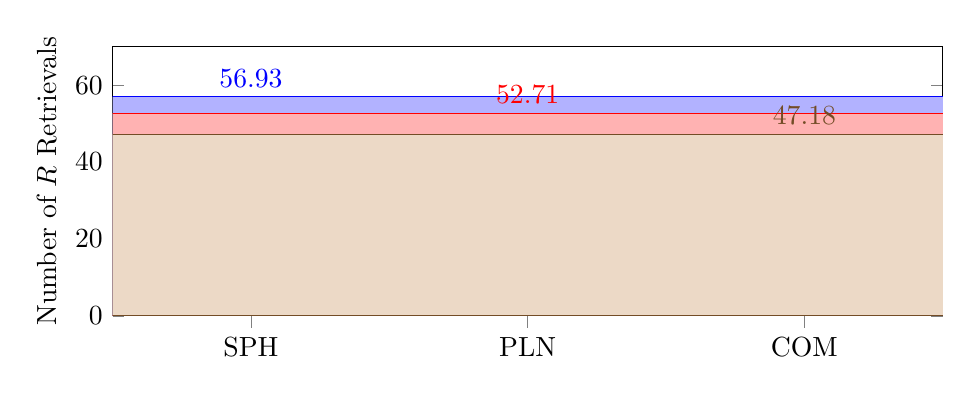
\begin{tikzpicture}
    \begin{axis}[
    ybar,
    width=\linewidth, height=5cm,
    ylabel={Number of $R$ Retrievals}, ylabel near ticks, ymin=0, ymax=70,
    xticklabels={SPH, PLN, COM},
    xtick={1, 2, 3}, xmin=0.5, xmax=3.5, xtick pos=left,
    nodes near coords, nodes near coords align={vertical},
    every axis plot/.append style={
    ybar,
    bar width=40,
    bar shift=0pt,
    fill
    }
    ]
        \addplot coordinates {(1, 56.93)}; % SPH
        \addplot coordinates {(2, 52.71)}; % PLN
        \addplot coordinates {(3, 47.18)};
    \end{axis}
\end{tikzpicture}

%SELECT AVG(QueryCount), IdentificationMethod
%FROM REDUCTION
%WHERE rowid IN (
%    SELECT rowid
%    FROM REDUCTION
%    WHERE (IdentificationMethod LIKE 'Plane' OR IdentificationMethod LIKE 'Sphere')
%    AND ShiftDeviation < 1.0e-3 AND ShiftDeviation > 1.0e-5 AND FalseStars = 0
%    AND QueryCount > 1
%)
%GROUP BY IdentificationMethod

%SELECT AVG(QueryCount)
%FROM REDUCTION
%WHERE rowid IN (
%    SELECT rowid
%    FROM REDUCTION
%    WHERE IdentificationMethod LIKE 'Composite'
%    AND ShiftDeviation < 1.0e-3 AND ShiftDeviation > 1.0e-5 AND FalseStars = 0
%    AND QueryCount > 1
%)
    \caption{
    Depicts the average number of database accesses required to obtain a $r$ set for strategies with triangular
    features given $\rho \seq \ang{0.0001}$ of Gaussian noise.
    To characterize the pivoting method itself, we only display instances where $\abs{R}\!\neq\!1$ with the first $b$
    selection.
%    The Spherical Triangle strategy has $1{,}952 / 2{,}000$ runs matching the criteria before, the Planar Triangle
%    strategy has $1{,}946$ runs, and the Composite Pyramid strategy has $1{,}957$ runs.
    }\label{fig:rPivot}
    }
\end{figure}

\subsubsection{How expensive is the pivoting process?}
%import numpy as np
%m_1, m_2, s_1, s_2, n_1, n_2 = 52.71, 47.18, 56.794658219949106, 47.01765577951369, 1946, 1957
%z = (m_2 - m_1) / np.sqrt( ((s_1 * s_1) / n_1) + ((s_2 * s_2) / n_2) )
As seen previously, identification strategies with triangular features have the most number of instances where
$\abs{R} \seq 1$ given an image with no noise.
~\autoref{fig:rPivot} displays the average number of database accesses for these same strategies where the first
$b$ selection does not meet the $R$ criterion given an image with Gaussian noise.
We note that the average number of database accesses is higher in strategies that use the pivoting processes,
as opposed to those that do not.
Given the null hypothesis that the difference between the Planar Triangle strategy's number of database accesses and
the Composite Pyramid strategy's number of database accesses is not significant, $z \seq 3.3, p\!<\!0.0001$ is
obtained with a two-tailed two sample $Z$ test.
With the data collected here, we find that the pivoting process results in more database accesses on average.
This increased number of database accesses results in a $6.70\si{ms}$ difference on average between the two.

The pivoting process was only tested with the strategies most frequently meeting the $R$ criterion.
An area of interest would be to see the effects of applying this process to strategies with angular features 
(i.e.\ Angle, Interior Angle, Pyramid).
These strategies met the criterion less frequently, and would likely benefit from attempting to reduce the $R$ set
before deciding to choose another $b$ set.

\subsection{Identification Step}\label{subsec:identificationStep}
\begin{figure}
    \centering{
        \begin{tikzpicture}
    \begin{axis}[
    ybar,
    width=\linewidth, height=5cm,
    ylabel={$a(h, b, r)$}, ylabel near ticks, ymin=0, ymax=1.3,
    xtick={1, 2, 3}, xticklabels={$\ang{0}$, $\ang{0.000001}$, $\ang{0.001}$},
    xlabel={$\sigma$ of Noise (degrees)}, xmin=0.5, xmax=3.5, xtick pos=left,
    nodes near coords, every node near coord/.append style={rotate=90, anchor=west},
    legend style={at={(0.5,-0.35)}, anchor=north,legend columns=-1},
    bar width=7
    ]
        \addplot coordinates {(1, 0.999416666666667) (2, 0.999222222222222) (3, 0.354333333333333)};
        \addplot coordinates {(1, 0.956083333333329) (2, 0.954444444444449) (3, 0.203166666666665)};
        \addplot coordinates {(1, 1.0) (2, 1.0) (3, 0.0)};
        \addplot coordinates {(1, 1.0) (2, 0.999833333333333) (3, 0.346333333333333)};
        \legend{PYR, PYR-N, COM, COM-N}
    \end{axis}
\end{tikzpicture}
        \caption{
        Depicts the frequency of correct bijections $a(h, b, r)$ formed with and without the verification step of
        both the Pyramid and Composite Pyramid strategies.
        There exists $2{,}000$ runs for each identification strategy, with a database access limit (i.e.\ number of 
        times the database is searched) of 500.
        The `-N' suffix indicates the strategy does not run with the verification step.
%        PYR corresponds to the Pyramid method with the verification step, PYR-N corresponds to the Pyramid method
%        without the verification step, COM corresponds to the Composite Pyramid method with the verification step,
%        and COM-N corresponds to the Composite Pyramid method without the verification step.
        }\label{fig:verify}
    }
\end{figure}

\begin{figure*} % HAD TO MOVE THIS GUY TOO...
    \centering{
    \begin{subfigure}[b]{0.48\linewidth}
        \begin{tikzpicture}
    \begin{axis}[
    ybar,
    width=\linewidth, height=5cm,
    ylabel={$t \ (\si{ms})$}, ylabel near ticks, ymin=10, ymax=100000,
    xtick={1, 2, 3}, xticklabels={$\ang{0}$, $\ang{0.0001}$, $\ang{0.01}$},
    xlabel={$\sigma$ (degrees)}, xmin=0.5, xmax=3.5, xtick pos=left, point meta=rawy,
    nodes near coords, every node near coord/.append style={rotate=90, anchor=west,
    /pgf/number format/.cd,fixed,precision=6},
    legend style={at={(0.5,-0.35)}, anchor=north,legend columns=-1},
    bar width=7, ymode=log, log origin=infty, max space between ticks=20
    ]
        \addplot coordinates {(1, 1197.43) (2, 1349.07) (3, 6509.00)};
        \addplot coordinates {(1, 160.68) (2, 161.80) (3, 872.22)};
        \addplot coordinates {(1, 323.94) (2, 339.23) (3, 392.29)};
        \addplot coordinates {(1, 324.35) (2, 328.85) (3, 352.24)};
        \addplot coordinates {(1, 170.79) (2, 171.53) (3, 364.04)};
        \addplot coordinates {(1, 405.53) (2, 1545.45) (3, 362.30)};
        \legend{ANG, INT, SPH, PLN, PYR, COM}
    \end{axis}
\end{tikzpicture}
    \end{subfigure}
    \begin{subfigure}[b]{0.48\linewidth}
        %if __name__ == '__main__':
%    from numpy import std, average, sqrt, polyfit, log
%    from sqlite3 import connect
%    from os import environ
%
%    conn_1 = connect(environ['HOKU_PROJECT_PATH'] + '/data/lumberjack-all-triad.db')
%    cur = conn_1.cursor()
%
%    # 1,   2,      3,      4,      5,     6,    7,   8
%    # 0.0, 1.0e-6, 1.0e-5, 0.0001, 0.001, 0.01, 0.1, 1.0
%
%    for d in [[1, 2, 3, 4, 5, 6, 7, 8], [0.0, 1.0e-6, 1.0e-5, 0.0001, 0.001, 0.01, 0.1, 1.0]]:
%        t = polyfit(log(d[3:]), [0.9725, 0.386, 0.0035, 0.0, 0.0], 1)
%        print('Angle: {}*ln(x) + {}'.format(t[0], t[1]))
%
%        t = polyfit(log(d[4:]), [0.9885, 0.7055, 0.033, 0.00383333333333333], 1)
%        print('Dot: {}*ln(x) + {}'.format(t[0], t[1]))
%
%        t = polyfit(log(d[2:]), [0.9715, 0.8135, 0.259, 0.0253333333333333, 0.0095, 0.00716666666666667], 1)
%        print('Sphere: {}*ln(x) + {}'.format(t[0], t[1]))
%
%        t = polyfit(log(d[2:]), [0.9865, 0.8615, 0.332166666666667, 0.0245, 0.0095, 0.00483333333333333], 1)
%        print('Plane: {}*ln(x) + {}'.format(t[0], t[1]))
%
%        t = polyfit(log(d[3:]), [0.999333333333334, 0.354333333333333, 0.0, 0.0, 0.0], 1)
%        print('Pyramid: {}*ln(x) + {}'.format(t[0], t[1]))
%
%        t = polyfit(log(d[1:]), [1.0, 0.65, 0.0035, 0.0, 0.0, 0.0, 0.0], 1)
%        print('Composite: {}*ln(x) + {}'.format(t[0], t[1])), print()

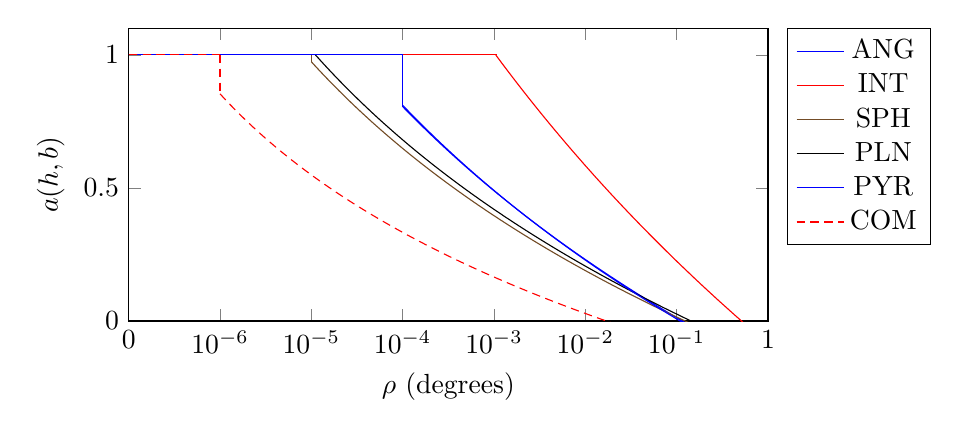
\begin{tikzpicture}
    \begin{axis}[
    width=0.8\linewidth, height=5.3cm,
    ylabel={$a(h, b)$}, ymin=0, ymax=1.1,
    xlabel={$\rho$ (degrees)}, xmin=1, xmax=8,
    xtick={1, 2, 3, 4, 5, 6, 7, 8},
    xticklabels={$0$, $10^{-6}$, $10^{-5}$, $10^{-4}$, $10^{-3}$, $10^{-2}$, $10^{-1}$, $1$},
    samples=100, no markers, legend pos=outer north east, enlargelimits=false
    ]
        \addplot +[domain=1:4, forget plot]{1};
        \addplot +[forget plot] coordinates {(4, 1) (4, 0.8055384229041530)};
        \addplot +[domain=4:8]{-1.416887591459587*ln(x) + 2.7697617012853217};
        \addlegendentry{ANG}

        \addplot +[domain=1:5.03, forget plot]{1};
%        \addplot +[forget plot] coordinates {(5, 1) (5, 1)};
        \addplot +[domain=5.02:8]{-2.3292306442173216*ln(x) + 4.757244753386215};
        \addlegendentry{INT}

        \addplot +[domain=1:3, forget plot]{1};
        \addplot +[forget plot] coordinates {(3, 1) (3, 0.9738787471803161)};
        \addplot +[domain=3:8]{-1.1317828984553227*ln(x) + 2.217269347527745};
        \addlegendentry{SPH}

        \addplot +[domain=1:3, forget plot]{1};
%        \addplot +[forget plot] coordinates {(3, 1) (3, )};
        \addplot +[domain=3.04:8]{-1.1696544292494204*ln(x) + 2.301996347627258};
        \addlegendentry{PLN}

        \addplot +[domain=1:4, forget plot]{1};
        \addplot +[forget plot] coordinates {(4, 1) (4, 0.8105837347641904)};
        \addplot +[domain=4:8]{-1.4347255837709008*ln(x) + 2.7995357213002334};
        \addlegendentry{PYR}

        \addplot +[domain=1:2, forget plot]{1};
        \addplot +[forget plot] coordinates {(2, 1) (2, 0.8533960244900531)};
        \addplot +[domain=2:8]{-0.7510156659772902*ln(x) + 1.3739604159185614};
        \addlegendentry{COM}
    \end{axis}
\end{tikzpicture}
    \end{subfigure}
    \caption{
    Both plots represent some statistic about the resulting bijection $h$ produced by each identification strategy
    given some image with varying Gaussian noise.
    There exist $2{,}000$ runs for each identification strategy, with a database access limit of 500.
    The left plot depicts the average time to obtain $h$, and the right plot depicts the trend line
    $a(h, b, r) = c \cdot \mathit{\ln}\left( \rho \right) + d$.
    }\label{fig:gaussianNoise}
    }
\end{figure*}

\subsubsection{How effective are additional verification steps?}
%if __name__ == '__main__':
%from numpy import std, average, sqrt
%from sqlite3 import connect
%from os import environ
%
%conn_1 = connect(environ['HOKU_PROJECT_PATH'] + '/data/lumberjack-all-triad.db')
%conn_2 = connect(environ['HOKU_PROJECT_PATH'] + '/data/lumberjack-pyramid-noverify.db')
%
%name = 'Pyramid'
%
%sample_1 = list(map(lambda b: b.execute("""
%SELECT PercentageCorrect
%FROM IDENTIFICATION
%WHERE ShiftDeviation < 1.0e-7 AND FalseStars = 0
%AND IdentificationMethod LIKE '{}'
%""".format(name)).fetchall(), [conn_1, conn_2]))
%
%sample_2 = list(map(lambda b: b.execute("""
%SELECT PercentageCorrect
%FROM IDENTIFICATION
%WHERE ShiftDeviation < 1.0e-5 AND FalseStars = 0
%AND IdentificationMethod LIKE '{}'
%""".format(name)).fetchall(), [conn_1, conn_2]))
%
%sample_3 = list(map(lambda b: b.execute("""
%SELECT PercentageCorrect
%FROM IDENTIFICATION
%WHERE ShiftDeviation < 1.0e-2 AND ShiftDeviation > 1.0e-4 AND FalseStars = 0
%AND IdentificationMethod LIKE '{}'
%""".format(name)).fetchall(), [conn_1, conn_2]))
%
%flatten = lambda a: [b[0] for b in a]
%for i, sample in enumerate([sample_1, sample_2, sample_3]):
%n_1, n_2 = 2000, 2000
%m_1, m_2 = average(flatten(sample[0])), average(flatten(sample[1]))
%s_1, s_2 = std(flatten(sample[0])), std(flatten(sample[1]))
%print('Z Score of {}: {}'.format(i, (m_2 - m_1) / sqrt( ((s_1 * s_1) / n_1) + ((s_2 * s_2) / n_2) )))

%import numpy as np
%print(np.average( [6.97725 - 3.00525, 6.9615 - 3.005, 398.0655 -  ))
In~\autoref{fig:verify}, the accuracy of the bijection produced by the Pyramid and Composite Pyramid strategies are
displayed with and without the verification step for varying levels of Gaussian noise.
Without noise, the Pyramid strategy without its verification step is 4.33\% less accurate than the Pyramid strategy with
verification on average.
This behavior is consistently seen for Gaussian noise of $\rho\seq\ang{0.000001}$ \& $\rho\seq\ang{0.001}$, and
can be attributed to the more frequent rejection of incorrect bijections with $R$ sets that have met the criterion.
In the $\rho\seq\ang{0.001}$ case, there exists a difference of 389.95 accesses between both variations of the Pyramid
and a 15\% bijection accuracy difference in favor of the strategy with the verification step.
Given the null hypotheses that the difference between both variations of the Pyramid strategy are different for each
level of noise, $z_0 \seq 15.87, z_{0.000001} \seq 16.04, z_{0.001} \seq 12.14$ (all $p\!<\!0.0001$) is obtained with
two-tailed two sample $Z$ tests.
The verification step increases the accuracy of the Pyramid strategy.

The response to Gaussian noise for the Composite Pyramid begins at $\rho\seq\ang{0.001}$, with a 34.6\% difference
between the two variants in favor of the strategy without the verification step.
Unlike the verification step in the Pyramid strategy, this filter appears to be too aggressive for the Composite Pyramid
strategy.
The variant without the verification step has an average of 193.93 database accesses at $\rho\seq\ang{0.001}$.
The Pyramid variant without the verification step only had an average of 8.114 database accesses, suggesting that the
$\abs{R} \seq 1$ criterion and the \Call{DMT}{} process are sufficient enough for rejecting incorrect $r$ sets and
bijections for the Composite Pyramid strategies.

\subsection{End to End}\label{subsec:endToEndEvaluation}
\subsubsection{Which strategy is the fastest given no noise?}
In~\autoref{fig:gaussianNoise}, the left plot depicts the end to end running time of each identification strategy given
varying degrees of Gaussian noise.
In the no noise case, the Angle strategy is the slowest identification strategy on average.
The next slowest strategy is the Composite Pyramid strategy, a factor of 2.95 times faster than the Angle strategy.
Recall that the Angle strategy had the fastest $R$ retrieval, but the largest $\abs{R}$.
On average, it takes 69.85 database accesses to obtain a bijection and 68.10 database accesses to obtain $r$.
This suggests that the Angle strategy's long running time stems from the $\abs{R} \seq 1$ criterion and not the
\Call{DMT}{} process.

%import numpy as np
%m_1, m_2, s_1, s_2, n_1, n_2 = 160.675, 170.7905, 0.53808, 0.52922, 2000, 2000
%z = (m_2 - m_1) / np.sqrt( ((s_1 * s_1) / n_1) + ((s_2 * s_2) / n_2) )
The fastest strategy in the no noise case appears to be the Interior Angle strategy, with the second fastest strategy
running 10.11\si{ms} slower.
There exists $0 / 2{,}000$ runs where the Interior Angle strategy runs above the Pyramid strategy's average running time
($170.79\si{ms}$) and the Interior Angle strategy has the fastest recorded identification run of 135ms.
The Interior Angle strategy is the fastest identification strategy given no noise.

\subsubsection{Which strategy is the fastest given varying levels of Gaussian noise?}
As Gaussian noise is increased from $\rho\seq\ang{0}$ to $\rho=\ang{0.01}$, the Angle strategy experiences the largest
response of $5{,}311.57$ additional $\si{ms}$.
The next slowest strategy in the noise of $\rho\seq\ang{0.01}$ case is the Interior Angle strategy, a factor of 7.46 times
faster than the Angle strategy.
On average, the Angle strategy takes 399.66 database accesses to obtain a bijection and only 36.72 database accesses
to obtain $r$ here.
In the no noise case, this strategy's long running time can attributed to the aggressive $R$ criterion.
Given Gaussian noise, the \Call{DMT}{} process plays a larger role with the Angle strategy and returns to $b$
decision process more often.

The Composite Pyramid strategy shows an interesting runtime response to this type of noise, running $1{,}139.92\si{ms}$
longer given $\ang{0.0001}$ of noise from no noise but $1{,}183.15\si{ms}$ shorter from $\ang{0.0001}$ of noise to
$\ang{0.01}$.
The Pyramid strategy is observed to have this same running time response against noise at $\rho\seq\ang{0.001}$
(not depicted).
The most probable explanation lies in how far each run travels from the $b$ decision step.
At $\rho\seq\ang{0.0001}$, the Composite Pyramid has gone through the $\abs{R} \seq 1$ criterion and is likely choosing
another $b$ set after the verification step.
At $\rho\seq\ang{0.01}$ the strategy is not passing the same criterion, avoiding the verification step.

%if __name__ == '__main__':
%from numpy import std, average, sqrt
%from sqlite3 import connect
%from os import environ
%
%conn_1 = connect(environ['HOKU_PROJECT_PATH'] + '/data/lumberjack-all-triad.db')
%conn_2 = connect(environ['HOKU_PROJECT_PATH'] + '/data/lumberjack-pyramid-noverify.db')
%
%sample_1 = conn_1.execute("""
%SELECT TimeToResult
%FROM IDENTIFICATION
%WHERE ShiftDeviation > 1.0e-7 AND FalseStars = 0
%AND IdentificationMethod LIKE 'Plane'
%""").fetchall()
%
%sample_2 = conn_1.execute("""
%SELECT TimeToResult
%FROM IDENTIFICATION
%WHERE ShiftDeviation > 1.0e-7 AND FalseStars = 0
%AND IdentificationMethod LIKE 'Pyramid'
%""").fetchall()
%
%flatten = lambda a: [b[0] for b in a]
%n_1, n_2 = 12000, 12000
%m_1, m_2 = average(flatten(sample_1)), average(flatten(sample_2))
%s_1, s_2 = std(flatten(sample_1)), std(flatten(sample_2))
%print('Z Score of: {}'.format((m_2 - m_1) / sqrt( ((s_1 * s_1) / n_1) + ((s_2 * s_2) / n_2) )))
The fastest strategy on average given images with Gaussian noise $\rho \in \set{10^{-1}, 10^{-2}, \ldots, 10^{-6}}$
is the Pyramid strategy at
$288.44\si{ms}$ (of 12,000 runs).
%\begin{equation}\label{eq:sigmasTested}
%    \rho \in \set{10^{-1}, 10^{-2}, \ldots, 10^{-6}}
%\end{equation}
The second fastest strategy given the same noise set is the Planar Triangle strategy at $341.16\si{ms}$.
Given the null hypothesis that the difference between both averages is not significant, $z \seq 24.32, p\!<\!0.0001$ is
found with a two-tailed two sample $Z$ test.
With the data collected here, the Pyramid strategy is the fastest strategy given varying amounts of Gaussian noise.

\begin{figure*}
    \centering{
    \begin{subfigure}[b]{0.48\linewidth}
        \begin{tikzpicture}
    \begin{axis}[
    ybar,
    width=\linewidth, height=5cm,
    ylabel={$t \ (\si{ms})$}, ylabel near ticks, ymin=10, ymax=100000,
    xtick={1, 2, 3}, xticklabels={0, 6, 12},
    xlabel={$\omega$}, xmin=0.5, xmax=3.5, xtick pos=left, point meta=rawy,
    nodes near coords, every node near coord/.append style={rotate=90, anchor=west,
    /pgf/number format/.cd,fixed,precision=2},
    legend style={at={(0.5,-0.35)}, anchor=north,legend columns=-1},
    bar width=7, ymode=log, log origin=infty, max space between ticks=20
    ]
        \addplot coordinates {(1, 1197.43) (2, 1737.94) (3, 2431.58)};
        \addplot coordinates {(1, 160.68) (2, 209.36) (3, 280.54)};
        \addplot coordinates {(1, 323.94) (2, 355.54) (3, 386.20)};
        \addplot coordinates {(1, 324.35) (2, 350.60) (3, 390.41)};
        \addplot coordinates {(1, 170.79) (2, 183.71) (3, 195.53)};
        \addplot coordinates {(1, 405.53) (2, 685.07) (3, 972.04)};
        \legend{ANG, DOT, SPH, PLN, PYR, COM}
    \end{axis}
\end{tikzpicture}
    \end{subfigure}
    \begin{subfigure}[b]{0.48\linewidth}
        \begin{tikzpicture}
    \begin{axis}[
    ybar,
    width=\linewidth, height=5cm,
    ylabel={Accuracy of Map, \texttt{ACC}}, ylabel near ticks, ymin=0, ymax=1.4,
    xtick={1, 2, 3}, xticklabels={0, 6, 12},
    xlabel={$\omega$}, xmin=0.5, xmax=3.5, xtick pos=left,
    nodes near coords, every node near coord/.append style={rotate=90, anchor=west,
    /pgf/number format/.cd,fixed,precision=4},
    legend style={at={(0.5,-0.35)}, anchor=north,legend columns=-1},
    bar width=7
    ]
        \addplot coordinates {(1, 0.977) (2, 0.979) (3, 0.960)};
        \addplot coordinates {(1, 1.0) (2, 0.982) (3, 0.965)};
        \addplot coordinates {(1, 1.0) (2, 0.840) (3, 0.696)};
        \addplot coordinates {(1, 1.0) (2, 0.845) (3, 0.703)};
        \addplot coordinates {(1, 0.999) (2, 0.999) (3, 0.995)};
        \addplot coordinates {(1, 1.0) (2, 0.994) (3, 0.973)};
        \legend{ANG, INT, SPH, PLN, PYR, COM}
    \end{axis}
\end{tikzpicture}
    \end{subfigure}
    \caption{
    Both plots represent some statistic about the resulting bijection $h$ produced by each identification strategy
    given some image with varying amounts of spikes $\omega$.
    There exist $2{,}000$ runs for each identification strategy, with a database access limit of 500.
    The left plot depicts the average time to obtain $h$, and the right plot depicts the average accuracy of $h$.
    }\label{fig:falseNoise}
    }
\end{figure*}

\subsubsection{Which strategy has the slowest growing $h$ accuracy response to increasing noise?}
The selection of the retrieval $\sigma$ parameters play a significant role in accuracy of each strategy given images
with Gaussian noise.
For strategies that search the database using on the $\theta$ feature (Angle, Interior Angle, Pyramid), the $\sigma$
parameter serves as a rough upper bound for the amount of Gaussian noise tolerated.
%In~\autoref{fig:gaussianNoise}, the plot on the right depicts the accuracy of resulting bijection of each method for
%varying levels of Gaussian noise.
When the level of noise is equal to the Angle and Pyramid $\sigma_\theta$ parameter ($\ang{0.0001}$),
both strategies have an average $h$ accuracy of $98.59\!\pm\!1.34\%$.
When Gaussian noise is increased to $\ang{0.001}$, both strategies drop to $47.02\!\pm\!1.58\%$.

For strategies with features that are not angular (Spherical Triangle, Planar Triangle, Composite Pyramid),
characterizing the effect of Gaussian noise becomes more difficult.
These strategies have the parameters $\sigma_a \seq 10^{-9}$ and $\sigma_\tau \seq 10^{-9}$, showing an initial
accuracy response to noise at $\ang{0.00001}$.
%The Interior Angle method has the largest query $\sigma$ parameters, and only experiences a response to noise at
%$\ang{0.01}$.
%Given the current set of query $\sigma$, the Interior Angle is the most accurate method on average.

Ranking each strategy based their $h$ accuracy is not particularly insightful here given the heavy dependence on
$\sigma$ parameters, so instead we analyze the rate of change involved with varying levels of noise.
The right plot in~\autoref{fig:gaussianNoise} depicts the trend line for all strategies where $h$ accuracy is displayed
against the amount of Gaussian noise.
It has been observed that the accuracy of each strategy remains near 100\% until it decreases exponentially to zero:
\begin{equation}
    a(f, b, r) =
    \begin{cases}
        0 & \rho < 0 \\
        1 & 0 \leq \rho < \rho^{\star} \\
        c \cdot \ln(\rho) + d & \rho \geq \rho^{\star}
    \end{cases}
\end{equation}
Each line was fit to the piecewise equation above ($c\cdot \ln(\rho) + d$ term with least squares), where $c$ and $d$
are the parameters found with the regression, $a(f, b, r)$ is the accuracy of the bijection, and $\rho^{\star}$ is the
point where $a(f, b, r)$ is observed to dip below 95\%.
The accuracy acceleration varies across strategies through the value of $c$:
\begin{equation}
    \frac{d^{2}a(f, b, r)}{d\rho^2} = \frac{-c}{\rho^2}
\end{equation}
A larger $c$ suggests that a change in retrieval $\sigma$ or Gaussian noise will not affect the accuracy of the strategy
as much as a strategy with a larger $c$.
The strategy with the largest acceleration toward $0\%$ $h$ accuracy is the Interior Angle strategy ($c \seq -0.15749$).
The Spherical Triangle strategy has the slowest growing $h$ accuracy response to increasing noise ($c \seq -0.09266$).

\subsubsection{Which strategy is the fastest given varying \\ amounts of false stars?}
In~\autoref{fig:falseNoise}, the plot on the left depicts the end to end running time of each strategy given varying
amounts of spikes.
As the number of spikes increases from 0 to 12, the Angle strategy again experiences the largest response of
$1{,}234.15\si{ms}$.
The next fastest strategy is the Composite Pyramid strategy, a factor of 2.50 times faster than the Angle strategy.
The difference between the 1st and 2nd slowest strategies is 2.98 times less than the Gaussian noise case.
On average, it takes 114.23 database accesses to obtain $h$ and only 54.85 accesses to obtain $r$.
Relative to the Gaussian noise comparison, \Call{DMT}{} and $\abs{R} \seq 1$ criterion play a more equal role in
the decision to choose a new $b$ set.

%if __name__ == '__main__':
%from numpy import std, average, sqrt
%from sqlite3 import connect
%from os import environ
%
%conn_1 = connect(environ['HOKU_PROJECT_PATH'] + '/data/lumberjack-all-triad.db')
%conn_2 = connect(environ['HOKU_PROJECT_PATH'] + '/data/lumberjack-pyramid-noverify.db')
%
%sample_1 = conn_1.execute("""
%SELECT TimeToResult
%FROM IDENTIFICATION
%WHERE FalseStars > 0
%AND IdentificationMethod LIKE 'Pyramid'
%""").fetchall()
%
%sample_2 = conn_1.execute("""
%SELECT TimeToResult
%FROM IDENTIFICATION
%WHERE FalseStars > 0
%AND IdentificationMethod LIKE 'Dot'
%""").fetchall()
%
%flatten = lambda a: [b[0] for b in a]
%n_1, n_2 = 8000, 8000
%m_1, m_2 = average(flatten(sample_1)), average(flatten(sample_2))
%s_1, s_2 = std(flatten(sample_1)), std(flatten(sample_2))
%print('Z Score of: {}'.format((m_2 - m_1) / sqrt( ((s_1 * s_1) / n_1) + ((s_2 * s_2) / n_2) )))
The fastest strategy on average given images with varying amounts of spikes is the Pyramid strategy at $186.22\si{ms}$.
The images given to each strategy contained $\omega$ spikes, where $\omega \in \set{ 3, 6, 9, 12 }$.
The second fastest strategy given the same noise set is the Interior Angle strategy at $228.37\si{ms}$.
Given the null hypothesis that the difference between both averages is not significant, $z \seq 28.47, p\!<\!0.0001$ is
found with a two-tailed two sample $Z$ test.
The Pyramid strategy is the fastest strategy given varying amounts of spikes.
The process for choosing distinct image star sets is shown to be effective in finding a bijection that meets the Pyramid
criteria the fastest.

%if __name__ == '__main__':
%from numpy import std, average, sqrt, polyfit, log
%from sqlite3 import connect
%from os import environ
%
%conn_1 = connect(environ['HOKU_PROJECT_PATH'] + '/data/lumberjack-all-triad.db')
%cur = conn_1.cursor()
%
%for name in ['Angle', 'Dot', 'Sphere', 'Plane', 'Pyramid', 'Composite']:
%sample_1 = list(map(lambda a: a[0], cur.execute("""
%SELECT AVG(TimeToResult)
%FROM IDENTIFICATION
%WHERE FalseStars > 0
%AND IdentificationMethod LIKE ?
%GROUP BY FalseStars
%ORDER BY FalseStars
%""", (name, )).fetchall()))
%
%t = polyfit([3, 6, 9, 12], sample_1, 1)
%print('{name}: {t_0}*x + {t_1}'.format(name=name, t_0=round(t[0], 5), t_1=round(t[1], 5)))
Each strategy exhibits a linear increase to runtime as additional spikes are added.
To characterize how each strategy's runtime grows with increasing false stars, each strategy's runtime was fit
to a linear equation using least squares:
\begin{equation}
    t = c\cdot\omega + d
\end{equation}
where $c$ and $d$ are the parameters found with the regression and $t$ is the end to end running time of the strategy.
A smaller $\abs{c}$ suggests that the number of spikes will affect the end to end runtime than that of a strategy with a
larger $\abs{c}$.
The strategy with the largest $\abs{c}$ is the Angle strategy with $c \seq -414.559$.
The strategy with the smallest $\abs{c}$ term is the Pyramid strategy with $c \seq -6.766$.
The Pyramid strategy is the fastest given varying amounts of false stars, having a runtime that is also the least
responsive to increasing spikes.

\subsubsection{Which strategy is the most accurate given varying amounts of false stars?}
%if __name__ == '__main__':
%from numpy import std, average, sqrt
%from sqlite3 import connect
%from os import environ
%
%conn_1 = connect(environ['HOKU_PROJECT_PATH'] + '/data/lumberjack-all-triad.db')
%conn_2 = connect(environ['HOKU_PROJECT_PATH'] + '/data/lumberjack-pyramid-noverify.db')
%
%sample_1 = conn_1.execute("""
%SELECT PercentageCorrect
%FROM IDENTIFICATION
%WHERE FalseStars = 12
%AND (IdentificationMethod LIKE 'Plane' OR IdentificationMethod LIKE 'Sphere')
%""").fetchall()
%
%sample_2 = conn_1.execute("""
%SELECT PercentageCorrect
%FROM REDUCTION
%WHERE FalseStars = 12
%AND (IdentificationMethod LIKE 'Plane' OR IdentificationMethod LIKE 'Sphere')
%""").fetchall()
%
%flatten = lambda a: [b[0] for b in a]
%n_1, n_2 = 2000, 2000
%m_1, m_2 = average(flatten(sample_1)), average(flatten(sample_2))
%s_1, s_2 = std(flatten(sample_1)), std(flatten(sample_2))
%print('Z Score of: {}'.format((m_2 - m_1) / sqrt( ((s_1 * s_1) / n_1) + ((s_2 * s_2) / n_2) )))
In~\autoref{fig:falseNoise}, the plot on the right depicts the average accuracy of each bijection given varying amounts
of spikes.
As the number of false stars is increased from $\omega \seq 0$ to $\omega \seq 12$, the strategies that experience
the largest $h$ accuracy response are the Spherical Triangle strategy ($30.42\%$ average decrease) and the Planar
Triangle strategy ($29.68\%$ average decrease).
The average accuracy of the $r$ selection is a few percent less than the average accuracy of $h$ here
($0.53\!\pm\!1.78\%$ for both strategies).
Given the null hypothesis that the difference between the accuracy of the $h$ bijection and the accuracy of the $r$
selection is not significant, $z \seq 0.37, p \seq 0.71$ was found with a two-tailed two sample $Z$ test.
There does not exist enough data to reject this hypothesis with $\alpha \seq 0.01$.
This suggests that the \Call{DMT}{} process is neither helpful or detrimental to the end to end accuracy of these
strategies.

Ruling out the \Call{DMT}{} process, the most likely source of error for the triangle strategies is their decision of
different $b$ sets.
If a false star exists as $b_1$ in $b$, the triangle strategies will have to iterate through $n^2$ combinations and
$n - 3$ pivots at most to choose another star that is not the spike.
The Angle strategy only has to wait $n$ additional combinations at most if a false star exists in $b$.
The Interior Angle strategy is able to get around the spike persistence problem by choosing $b$ sets based on their
$\theta$ proximity to the central star $b_c$.
The Pyramid and Composite Pyramid strategies have their $b$ decision process designed for this situation, increasing the
average turnover of all stars in the $b$ set.

The Pyramid strategy has the most accurate $h$ on average given images with all different $\omega$ at $99.84\!\pm\!3.53\%$.
The second most accurate strategy is the Composite Pyramid strategy at $99.19\!\pm\!8.95\%$.
Given the null hypothesis that the difference between the $h$ accuracies of both strategies is not significant,
$z \seq 3.02, p \seq 0.003$ with a two-tailed two sample $Z$ test.
At $\alpha \seq 0.01$, our hypothesis does not hold true.
The Pyramid strategy is the most accurate under varying amounts of spikes.
